% change according to folder and file names
\ifpdf
    \graphicspath{{4/figures/PNG/}{4/figures/PDF/}{3/figures/}}
\else
    \graphicspath{{4/figures/EPS/}{4/figures/}}
\fi

%: ----------------------- contents from here ------------------------
\chapter{EAs and MAEAs Supported by Principal Component Analysis} % top level followed by section, subsection
\label{VarCorrChapter}
%\begin{flushright}
%Any intelligent fool can make things  
%\linebreak
%bigger, more complex, and more violent. 
%\linebreak
%It takes a touch of genius, and a lot of  
%\linebreak
%courage, to move in the opposite direction.
%\linebreak
%Albert Einstein
%\end{flushright}

This chapter investigates the reasons for the efficiency degradation of EAs or MAEAs used to solve ill-posed optimization problems \cite{Salomon,Roy_2002a,Ghisu_2010}, specially when they are combined with a great number of N, and proposes techniques to avoid it. Any degradation in the EAs or MAEAs efficiency reflects upon the number of evaluations (on the CFD software, for instance) required to reach the optimal solution(s).  Increasing the number of evaluations leads to longer optimization turn around times and the routine application of EA-based optimization in large-scale industrial applications is thus hindered. The proposed methods adapt the application of the evolution operators accordingly (for use in EAs and MAEAs) and/or assist in training more dependable metamodels on patterns of properly reduced dimension (for use in MAEAs).

Modern industrial-scale optimization problems typically have several objectives and/or constraints with complex parameterization and a great number N of design variables. The former is determined by the application under consideration whereas the latter is, often, ``inherited'' from the way experienced designers used to accomplish the same task in the past, without resorting to ``sophisticated'' optimization methods. From the practical point of view, a smooth transition to the EA-based optimization is necessary. Problems with several objectives and/or constraints which handle many design variables can easily become ill-posed, as discussed in section \ref{illpost}. The use of stochastic population-based search methods to solve ill-posed problems leads to excessively long computations, even on multi-processor platforms. Since the objectives and the constraints are strictly defined by the application, the only way to increase the efficiency of EAs used to solve ill-posed optimization problems is via the appropriate handling of the parameterization. 

Changing the parameterization, though, may have a number of negative effects. First among them is that, in any industrial environment, a valuable amount of experience is embodied into the existing parameterization, in the sense that an experienced designer practically knows exactly what to change in order to achieve a given goal; this will be lost by altering the paremeterization scheme. Also, there is no guarantee that the parameterization which must be built in accordance with the objectives so as to give a better-posed optimization problem, includes variables with a clear interpretation (being, for instance, the coordinates of \Bezier\ control points, etc.), in fact this is highly unlikeable. The new parameterization, lacking a clear interpretation of the design variables, deems the accumulation of new experience impossible. Furthermore, for a specific project, the best parameterization depends on its correlation with the corresponding  objectives and constraints. Therefore, a different parameterization would be necessary for any new design-optimization procedure, based on its objectives. To make things even worse, the best parameterization cannot be known in advance, since one should have the Pareto front available so as to get a good idea about the shape of the scalar cost function in the design space and use it for extracting the most appropriate parameterization. All the above cane be overcome by implementing the techniques proposed in this chapter.                 


The fact that, a standard GA can find the global optimum in a number of widely used test functions was not only due to the efficiency of the recombination operator and the regular distribution of local minima, but also because the test functions were decomposable was presented in \cite{Salomon}. Though \citep{Salomon} was based on a GA, its outcomes can be generalized for any EA. In \cite{Roy_2002a,Roy_2002b},  it was stated that ``real-life'' engineering design optimisation problems, as opposed to the widely used mathematical test cases also involve ``interactions among design variables''. There, \cite{Roy_2002a,Roy_2002b}, the notions of ``inseparable function interaction'' and ``variable dependence'' were introduced. These ``variable dependence'' pose a number of challenges for multi-objective optimisation algorithms and is equivalent to the so called ill-posed optimization problem as defined in this thesis.
Also, as stated in \cite{Roy_2002b}, depending upon the nature of ``variable dependency'', additional features such as bias (non-linearity), multi-modality, deception and discontinuity may also occur and these will cause efficiency degradation of the optimization algorithm. 


%  In \cite{Ghisu_2010}, the merits of adaptive parameterization in MOO with taboo search.



%In the same context with ill-posed optimization problems but with different phrasing significant work has been done by Ralf Salomon, Rajkumar Roy and Tiziano Ghisu. 
%Ralf Salomon presented, in \cite{Salomon}, the efficiency degradation of GAs if the same optimization problem was posed in a ``non-decomposable'' way. Later, Rajkumar Roy presented the, in \cite{Roy_2002a}, the notions of ``Inseparable Function Interaction'' and ``Variable Dependence''. Tiziano Ghisu, in \cite{Ghisu_2010}, presented the merits of adaptive parameterization in MOO with taboo search. 

 

\section{Ill-posed optimization problems}
\label{illpost}
The two main reasons for increasing the number of calls to the evaluation software  required by an EA or MAEA in order to locate the optimal solution(s) are; a) the high number of design variables, $N\!>>$ and b) the fact that an ill-posed optimization problem is to be solved. Needless to say that a high-dimensional ill-posed optimization problem is the worst case for an EA or MAEA.  Unfortunately, in practice, most engineering optimization problems share both the aforementioned features. 

In EAs the high number of design variables (N) can cause efficiency deterioration. In the best case (well-posed problem) the computational cost for computing the optimal design(s) increases linearly with N. In MAEAs, the presence of $N\!>>$ design variables, apart from the way the optimal solution is approached (direct effect), also affects the use of metamodels for which the training time and, mainly,  prediction error increase noticeably. The loss in efficiency due to the ``less-accurate'' metamodel predictions (indirect effect) is, practically, superimposed to the performance degradation due to the direct effect.  As a remedy to the class of optimization problems with $N\!>>$, the KBD method was proposed in Chapter 3. The KBD method reduces the problem dimension by exploiting the knowledge embodied into a small number of available archived designs and has already been presented and validated in chapter 3.             

On the other hand, ill-posed optimization problems are those dealing with; (a) anisotropic and (b)  non-separable objective function f. Let us note that (a) is a prerequisite for (b). In fact the term ill-posed optimization problem is equivalent to an optimization problem which deals with a non-separable objective function. The definitions of anisotropic and non-separable functions follow in sections \ref{IllCon} and \ref{Nonsep}, respectively. Ill-posed problems, in combination with $N\!>>$, give rise to the so called ``curse of dimensionality''. This stands for the situation in which the cost for solving an optimization problem increases superlinearly, instead of just linearly, with N. 
% Thus an ill-post optimization problem, when solved with EAs, is magnifying the negative effects of big N. 

%Herein the definitions of a) anisotropic objective function and b) non-separable objective function that characterize the objective function of an ill-posed problem are presented. Later, an investigation regarding the effects of ill-posed optimization problems on EA efficiency is carried out.  

\subsection{Anisotropic objective function}
\label{IllCon}
%The term anisotropic objective function refers to the condition were the contribution to the objective function value is largely anisotropic for the different design variables or ,more precisely, directions in search space.
An objective function $f(\vec{x})$, $\vec{x}=(x_1,...,x_N)$  is anisotropic with respect to $\vec{x}$ if this is differently affected by the same changes in the different components of $\vec{x}$. Though this thesis is dealing with non-gradient-based optimization methods, the anisotropy of f can be quantified by the variation of $\frac{\partial f}{\partial x_i}$ among $i$ close to the optimal solution. 

%This variation, and thus the magnitude of anisotropy, can be quantified via the condition number (a) of the Hessian matrix (H).


For instance, for the convex-quadratic function
\begin{eqnarray}
   f(\vec{x}) = \frac{1}{2}\vec{x}^TH\vec{x}
   \label{conv.1}
\end{eqnarray}
considered as the objective function of an optimization problem. Where $H$ is a symmetric positive definite $N \times N$ matrix,
the variation in $\frac{\partial f}{\partial x_i}$  is expressed by the condition number a of the Hessian matrix H. $a$ is defined as the ratio of H's largest and smallest eigenvalue. 
These two eigenvalues correspond to the squared relative lengths of the principal axes of the ellipsoid $\vec{x}^TH\vec{x} = 1$. For points located along the principal axes, the gradient aligns with the axis itself, and the ellipsoid-axis length determines the magnitude of movement required to achieve a certain change in f. Therefore, function f is said to be isotropic if the condition number of $H$ is $a=1$ (corresponding to a sphere or hyper-sphere, see fig. \ref{illc}) and anisotropic if $a\!>>\!1$ (corresponding to an ellipse, see fig. \ref{illc}).

  


\begin{figure}[h!]
\begin{minipage}[b]{1.0\linewidth}
 \centering
 \resizebox*{15cm}{!}{
\includegraphics{ellipseA.eps}}
\end{minipage}
%\begin{minipage}[b]{0.5\linewidth}
% \centering
% \resizebox*{7.5cm}{!}{
\includegraphics{ellipseA.eps}}
%\end{minipage}
\caption{Iso-value contours of an isotropic objective function with two design variables (left); the contribution of both $x_1$ and $x_2$ in f are the same. Iso-value contours of an anisotropic objective function; in which variable $x_2$ has higher contribution to the objective function than $x_1$ (right).} 
\label{illc}
\end{figure}

In practice, EAs are capable to efficiently deal with anisotropic objective functions without damaging their efficiency. If, however, the objective function is anisotropic and non-separable (see definition in section \ref{Nonsep}), the EA or MAEA is expected to worsen its efficiency, unless a particular treatment is employed; such a treatment is proposed in this thesis.  

Furthermore, the anisotropy of f leads to the notion of more and less important design variables (or, in the case of non-separable f, more and less important directions in the design space). This piece of information can be used to reduce N, via the artificial truncation of the less important variables during the metamodel training phase, so as to increase its prediction ability.       


\subsection{Non-separable objective function}     
\label{Nonsep}
The separability of an objective function $f:\vec{x}\mapsto f(\vec{x})$ is defined separately for each and every variable $x_i \in \vec{x}$. An objective function is said to be separable with respect to $x_i$ if the optimal value of $x_i$ does not depend on the value  any other design variable takes on. $f$ is said to be separable if and only if is separable with respect to all components of $\vec{x}$.


\begin{figure}[h!]
\begin{minipage}[b]{1\linewidth}
 \centering
 \resizebox*{14cm}{!}{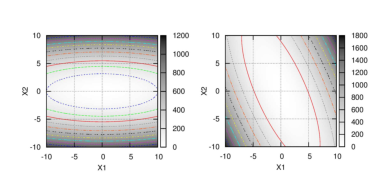
\includegraphics{ellipseB.eps}}
\end{minipage}
%\begin{minipage}[b]{0.5\linewidth}
% \centering
% \resizebox*{9cm}{!}{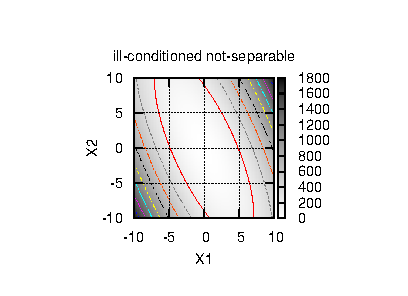
\includegraphics{ellipseturn.eps}}
%\end{minipage}
\caption{Left: Separable objective function. Right: Non-separable objective function.} 
\label{nonsep}
\end{figure}

As mentioned above an ill-posed optimization problem suffers from the curse of dimensionality, the computational cost to solve it scales superlinearly with the number of design variables N. This caused by the presence of a non-separable objective function. To better understand this, let us first examine a separable objective function. The cost for solving an optimization problem with a separable objective function increases linearly with N, since the global optimum can be located by minimizing $N$ objective functions with a single design variable each (separately minimise $f_i(x_i),~ \forall x_i \in \vec{x}$). Thus, the cost to solve a separable $N$-dimensional optimization problem is approximately $N$ times the cost to solve the equivalent 1D problem. On the other hand, this is not possible for an ill-posed optimization problem, since, for at least one design variable, its optimal value depends on the values the rest take on. Furthermore, regarding the ill-posed problem, the search space increases exponentially with N and therefore the cost of solving the ill-posed optimization problem increases superlinearly with N.   
 
\subsection{Investigation of EA efficiency degradation when solving ill-posed optimization problem}
\label{Inv2}

In order to Investigate the effects of ill-posed optimization problems on EA efficiency, two mathematical test cases are solved, with different N values, both in their separable (well-posed) and non-separable (ill-posed) form. All the results presented in this section correspond to the mean performance over $10$ runs, with different random number generator seeds. 

The first analytical test case to be examined is a multi-dimensional ellipsoid (a 2D version of it can be seen in fig. \ref{nonsep}) described, in its separable form, by:   


\begin{eqnarray}
   f(\vec{x})=\sum^{n}_{i=1} a^{\frac{i-1}{n-1}}x_i^2
   \label{ellipse} 
\end{eqnarray}
where the value of the coefficient $a$ determined the anisotropy of the objective function. Large values of $a$ lead to increasingly anisotropic objective functions.

The same problem can be examined after casting it in its non-separable form by, as follows

\begin{eqnarray}
   f(\vec{x})=\sum^{n}_{i=1}a^{\frac{i-1}{n-1}}y_i^2
   \label{ellipse} 
\end{eqnarray}
where $\vec{y}=B\vec{x}$ and $B$ is a $n\times n$ orthogonal rotation matrix.

In order to investigate both the effects of the design space dimension ($N$) and the condition number ($a$), four different optimization problems will be solved. A ten dimensional ($N\!=\!10$) optimization problem is solved for $a\!=\!10$ and $a\!=\!100$, see fig. \ref{ellipse_t1}, and a $n\!=\!30$ problem is solved for $a\!=\!100$ and $a\!=\!1000$, see fig. \ref{ellipse_t2}. 


\begin{figure}[h!]
\begin{minipage}[b]{0.5\linewidth}
 \centering
 \resizebox*{7.5cm}{!}{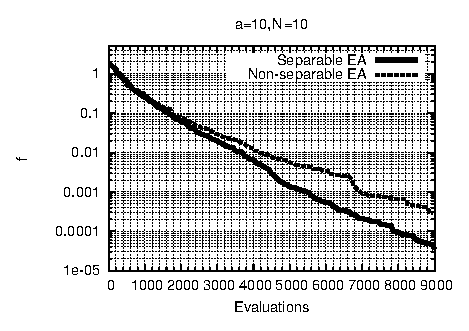
\includegraphics{10_10d.eps}}
\end{minipage}
\begin{minipage}[b]{0.5\linewidth}
 \centering
 \resizebox*{7.5cm}{!}{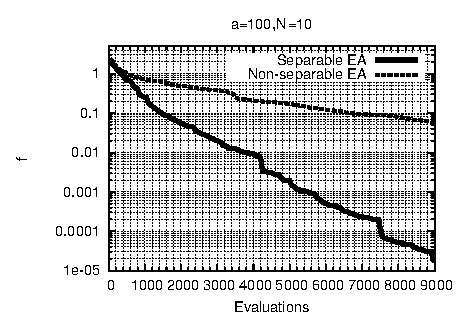
\includegraphics{100_10d.eps}}
\end{minipage}
\caption{10D ellipsoid. Left: condition number $a\!=\!10$.  Right: condition number $a\!=\!100$. Increasing $a$ from $10$ to $100$  increases the performance gap between the separable and non-separable problem.} 
\label{ellipse_t1}
\end{figure}

\begin{figure}[h!]
\begin{minipage}[b]{0.5\linewidth}
 \centering
 \resizebox*{7.5cm}{!}{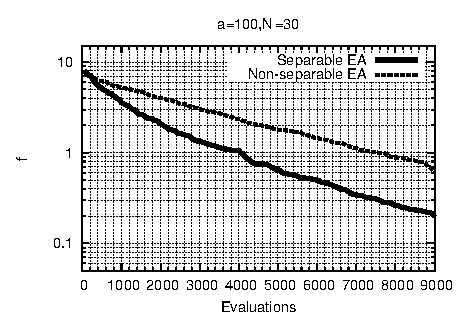
\includegraphics{100_30d.eps}}
\end{minipage}
\begin{minipage}[b]{0.5\linewidth}
 \centering
 \resizebox*{7.5cm}{!}{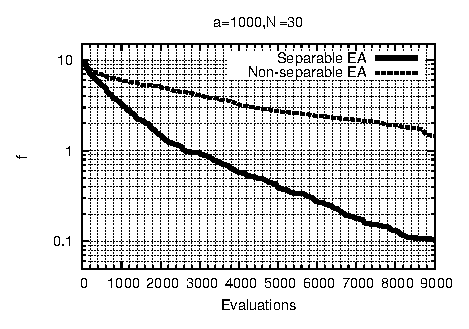
\includegraphics{1000_30d.eps}}
\end{minipage}
\caption{30D ellipsoid. Left: condition number $a\!=\!100$.  Right: condition number $a\!=\!1000$. Increasing of $a$ from $100$ to $1000$, as in the 10D case, causes additional losses and increases the performance gap between separable and non-separable optimization problem.} 

\label{ellipse_t2}
\end{figure}

In figs. \ref{ellipse_t1} and \ref{ellipse_t2} one can identify both the effects of increasing the condition number and increasing the problem dimension. A condition number with higher value leads to greater performance gap between the separable and non-separable cases, for both the $N\!=\!10$ and $N\!=\!30$ cases. Increasing the problem dimension also increases the gap between the two. Focusing on the $a\!=\!100$ case, for both the $N\!=\!10$ and $N\!=\!30$ one may observe that the difference of objective function values $\Delta(f)$, for the same computational cost of $9000$ evaluations, differ. For the $N\!=\!10$ case $\Delta(f)\!=\!f(non-separable)-f(separable) \approx  10^{-4}$. On the other hand, for the $n=30$ case $\Delta(f)\!=\!f(non-separable)-f(separable) \approx  0.9$. This difference in $\Delta(f)$ for the 10D and 30D cases denotes a significant increase of the efficiency gap between separable and non-separable cases when the dimension is increased.      

The second analytical test case has a multi-modal objective function described by  

\begin{eqnarray}
   f(\vec{x})=10N+(\sum^{N}_{i=1}x_i)^2 - 10N~ cos(\pi  \sum^{N}_{i=1}x_i)
   \label{mm} 
\end{eqnarray}

A 2D example of it is shown in fig. \ref{multimod}. As it appears in the eq. \ref{mm}, the problem is non-separable. It can though easily be transformed to a separable one if $\vec{x}$ is transformed into $\vec{y}=B\vec{x}$ where $B$ the appropriate rotation matrix.  In each direction, a $45^o$ rotation is employed.  This objective function can also is extremely anisotropic since only one direction is the design space has contribution in the objective faction value and all the rest became irrelevant therefore the condition number $a$ equals practically to $\infty$. This is an important class of objective functions since it resembles MOO problems as we will see further on (section \ref{VCMM}).    

In order to investigate the effects of non-separability as a function of the problems dimension two optimization problems where solved a $5$ and a $30$ dimensional one.  
\begin{figure}[h!]
\begin{minipage}[b]{1\linewidth}
 \centering
 \resizebox*{14cm}{!}{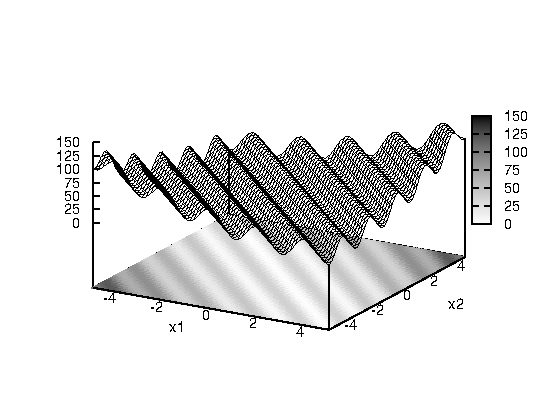
\includegraphics{multimodnomap.eps}}
\end{minipage}
%\begin{minipage}[b]{1\linewidth}
 %\centering
 %\resizebox*{11cm}{!}{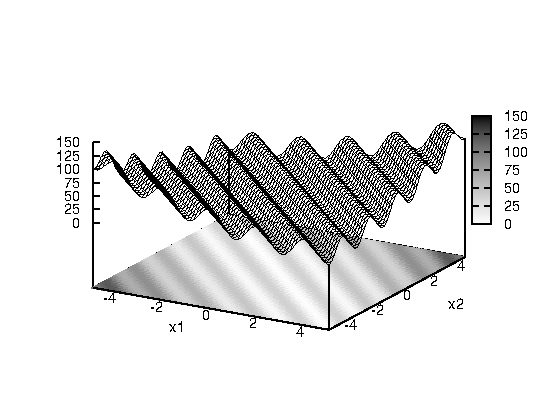
\includegraphics{multimodnomap.eps}}
%\end{minipage}
\caption{Minimization of eq. \ref{mm}, 2D graphical representation. The optimal value of $x_1$  depends on the choice of $x_2$ and vice-versa thus this objective function is non-separable. Nevertheless, if one of the two design variables was aligned to the $x_1=x_2$ axis, the problem becomes separable.} 

\label{multimod}
\end{figure}

In fig. \ref{multimodres}, it is demonstrated that for either the 5D or 30D problem, the reformulated problem with a separable objective function outperforms the case with the non-separable one. Furthermore, one may observe that by increasing the problem dimension caused an increase in the efficiency gain, between separable and non-separable function cases. This conclusion is similar to the one made for the ellispoid test case. 



\begin{figure}[h!]
\begin{minipage}[b]{0.5\linewidth}
 \centering
 \resizebox*{7cm}{!}{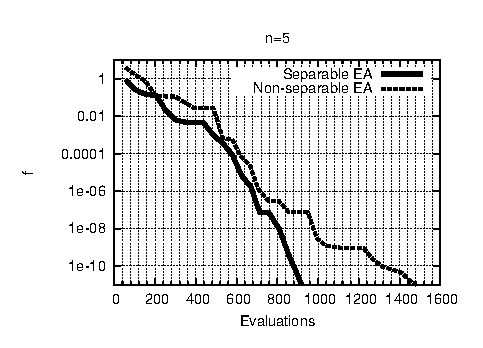
\includegraphics{5d.eps}}
\end{minipage}
\begin{minipage}[b]{0.5\linewidth}
 \centering
 \resizebox*{7cm}{!}{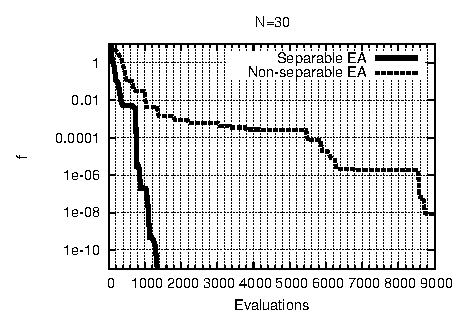
\includegraphics{30d.eps}}
\end{minipage}
\caption{Left: 5D problem of eq.\ref{mm}. Right: 30D problem of eq.\ref{mm}. The loss in efficiency for problems with extremely anisotropic objective functions increases significantly with the design space dimension.} 
\label{multimodres}
\end{figure}

Through the preformed investigations  (figs. \ref{ellipse_t1}, \ref{ellipse_t2} and \ref{multimodres}) it is convincingly shown  that a significant amount of the EA efficiency can be lost when dealing with ill-posed optimization problems. The degree of efficiency deterioration is proportional to three quantities;

\begin{description}
  \item[a)] The anisotropy magnitude. Increasing anisotropy leads to a more inefficient EA(figs. \ref{ellipse_t1} and \ref{ellipse_t2}).    
  \item[b)] Function separability. Optimization problems with separable objective functions with respect to their design variables can be solved significantly faster using EAs, as shown in figs. \ref{ellipse_t1}, \ref{ellipse_t2} and \ref{multimodres}.  
  \item[c)] The number of design variables $N$. It is obvious that by increasing the number of design variables any EA requires more computational resources to locate the optimal solution. Additionally, if combined with b), the great value of $N$ leads to the so-called curse of dimensionality (fig. \ref{multimodres}).  
\end{description}

\section{Ill-posed MOO problems}
\label{VCMM}
Regarding ill-posed MOO problems one should observe $\Phi$, since $\Phi$ is the quantity that drives the evolution operators. In MOO, ill-posed optimization problem are typically in the form of non-separable extremely anisotropic. This results from the fact that a Pareto front of optimal non-dominated solutions is sought. Since the assignment of $\Phi$ on Pareto dominance, all members of the current front of non-dominated solutions have $\Phi=0$ (or very small values compared to the dominated members of the population).

\section{Improved Parameterization}
The aim is to find the appropriate linear orthogonal transformation of the original set of design variables $\vec{x}  \rightarrow \vec{x}^*$ which will transform the ill-posed optimization problem in hand into a well-posed one. In specific after this transformation the objective function (SOO) or $\Phi$ (MOO) is expected to has enhanced separability with respect to the transformed design variables $\vec{x}^*$.  This procedure is equivalent to finding an orthogonal matrix $U$ ($UU^T=I$) and express the transformed $\vec{x}^*=U^T\vec{x}$. The latter equation stands for a simple coordinate system rotation where that the new basis is the $\vec{x}^*$. In this thesis, it is said that the topological characteristics of the Pareto front indicate the appropriate transformation matrix $U$.  To extract the topological characteristics of the Pareto front in a way which best represents the data variance, principal component analysis (PCA) is used ,\cite{Hayk1999,Jolliffe_2002}. Therefore, the transformation matrix $U$ is said to be the matrix which contains the Principal Directions (PDs) as they were computed by the PCA applied on the members of the Pareto front.   

As shown earlier in this chapter, switching form $\vec{x}$ to $\vec{x}^*$ and by applying the evolution operators on that, can lead to a significantly faster exploration of the design space. However, this requires the knowledge of the Pareto front, the finding of which is the final goal of the optimization process.  Instead, in each EA generation, the front of non-dominates solutions (elite-set) can be used for the PCA. This is a reasonable choice since, as the evolution proceeds, the current elite-set tents to the Pareto front. Thus, PDs computed based on the elite-set are, increasingly reliable, approximations of the PDs computed based on the Pareto front.

Applying PCA to the current elite-set first demands the transformation of  its members into a standardized data-set ($X$) with $\mu=0$ and $\sigma=1$ in all directions. Next step is the empirical covariance matrix $P$, \cite{Fodor_2002, Jolliffe_2002} computation,

\begin{equation} 
   P_{N\times N}= \frac{1}{e}XX^T
   \label{Cov_Mat} 
\end{equation}

where $e$ is the size of the elite set and $X$ the matrix which contains the members of the elite-set as columns. Then via the spectral decomposition theorem, \cite{Axler_1997, Fodor_2002}, $P$ can be written as

\begin{equation} 
   P_{N\times N}= U\Lambda U^T
   \label{spectral}
\end{equation}
where $\Lambda\!=\!diag(\lambda_1 , . . . , \lambda_N )$ is the diagonal matrix with the eigenvalues of $P$ and $U$ is a $N\!\times\!N$ matrix formed containing the eigenvectors (PDs) as columns. 


In industrial scale optimization problems, such as the ones this thesis is dealing with, where the evaluation of a candidate solution may cost from minutes up to even hours on a multiprocessor system, the additional computational cost attributed to the PCA computation is, practically, negligible.


The most efficient method to perform PCA is by means of the so-called singular value decomposition (SVD), \cite{press_etal:1992}, which allows the matrix $X$ to be expressed as

\begin{equation} 
   X = U\Lambda V^T
   \label{Cov_Mat2} 
\end{equation}

where, $V^T$ a matrix containing the eigenvectors of $X^TX$.

In industrial scale optimization problems, such as the ones concerning this thesis, where a design evaluation requires time of the order of minutes or even hours, the portion of the total computational cost attributable to PCA computation is negligible.
 


To better demonstrate the variable correlation estimation in MOO problems  the welded beam test case is used (fig. \ref{case}).  The minimization of both the cost ($K$) and the deflection ($\Delta$) of a welded beam subject to a force $P$ (fig. \ref{case}) is desired. There are two design variables: the welding length ($X_1$)  and the side length of the square cross section ($X_2$) (fig. \ref{case}). The design is subject to constraints of shear stress ($\tau$), bending stress ($\sigma$) and buckling load ($P_c$).    

\begin{figure}
\begin{minipage}[b]{1\linewidth}
 \centering
 \resizebox*{5cm}{!}{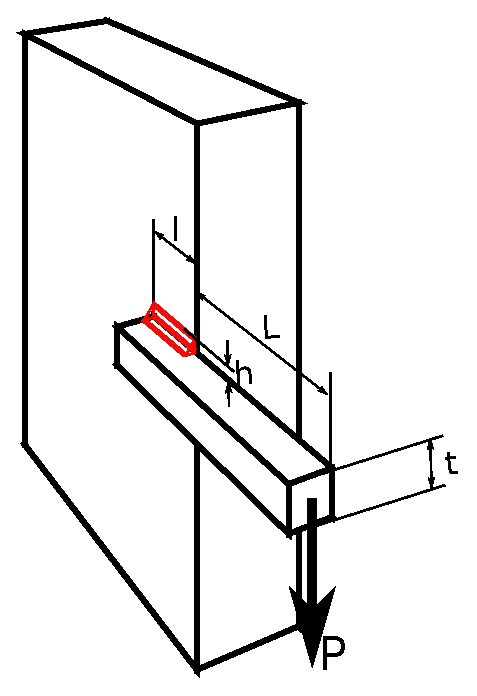
\includegraphics{case.eps}}
\end{minipage}
\caption{In the examined case, design variables are square cross section side-length ($X_2 = t$) and welding length ($X_1 = l$) are the design variables.} 
\label{case}
\end{figure}

%\figuremacroW{case}{Welded beam case - Problem definition.}{In the examined case, design variables are square cross section side-length ($X_2 = t$) and welding length ($X_1 = l$) are the design variables.}{0.4}

The problem is formulated formulated as,

Minimize Cost,
%\begin{equation} 
\begin{eqnarray}\nonumber
   K = 1.10471h^2l+0.04811t^2(14.0+l) \\
   = 1.10471h^2X_1+0.04811X_2^2(14.0+X_1)
   \label{Cost} 
\end{eqnarray}
and minimize Deflection,
%\end{equation}
\begin{eqnarray}
   \Delta = \frac{4PL^3}{Et^4} = \frac{4PL^3}{EX_2^4}
   \label{Deflection} 
\end{eqnarray}

Subject to:


Constraint concerning the shear stress applied on the welding in order to ensure the structural integrity of the welding. Maximum shear stress depends on the type and quality of the welding. 
\begin{eqnarray}
   \tau = \sqrt{\tau_1^2 + \frac{\tau_1 \tau_2 l}{R} +\tau_2^2} \\
   \nonumber \tau \leq 13,600 psi \\
   \nonumber where:~~~~~~~~~~~~~~~~~~~~~~.\\
   \nonumber \tau_1 = \frac{P}{\sqrt{2}hl} \\
   \nonumber \tau_2 = \frac{MR}{J} \\   
   \nonumber M = P(L+\frac{l}{2}) \\ 
   \nonumber R = \sqrt{\frac{l^2}{4} + (\frac{h+t}{2})^2} \\
   \nonumber J = 2\left( \sqrt{2}hl\left( \frac{l^2}{12} + \left(\frac{h+t}{2}\right)^2 \right) \right)
   \label{shear} 
\end{eqnarray}

concerning the bending stress applied on the beam, to ensure structural integrity of the beam. Maximum bending stress depends on the beam material.
\begin{eqnarray}
   \sigma = \frac{6PL}{t^3} \leq 30,000 psi
   \label{bend} 
\end{eqnarray}

and concerning the buckling load, to avoid buckling phenomena.  
\begin{eqnarray}
   P_c = \frac{4.013E\sqrt{\frac{t^8}{36}}}{L^2}\left( 1- \frac{t}{2L}\sqrt{\frac{E}{4G}} \right) \\
   \nonumber  P - P_c \leq 0 
   \label{back} 
\end{eqnarray}
where welding hight is $h = 0.6 in$, beam reach is $L = 14 in$, the extend of the force is $P = 6000 lb$, Young’s modulus is $E = 30 \times 10^6 psi$, and shear modulus is $G = 12 \times 10^6 psi$.  

Apart from the structural, constraints are also enforced on the objectives to bound the Pareto front within logical values, thus:

\begin{eqnarray}
   K \leq 50 \\
   \Delta \leq 0.25 
   \label{obj} 
\end{eqnarray}


\begin{figure}[h!]
%\begin{minipage}[b]{0.5\linewidth}
% \centering
% \resizebox*{7cm}{!}{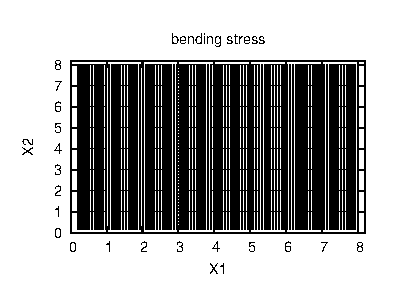
\includegraphics{Const_sx.eps}}
%\end{minipage}
%\begin{minipage}[b]{0.5\linewidth}
% \centering
% \resizebox*{7.5cm}{!}{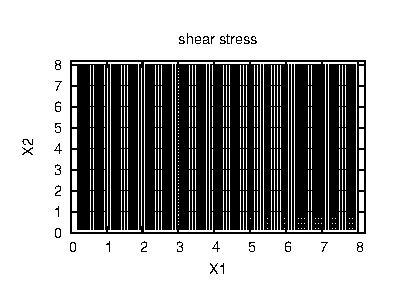
\includegraphics{Const_tx.eps}}
%\end{minipage}
%\begin{minipage}[b]{0.5\linewidth}
% \centering
% \resizebox*{7.5cm}{!}{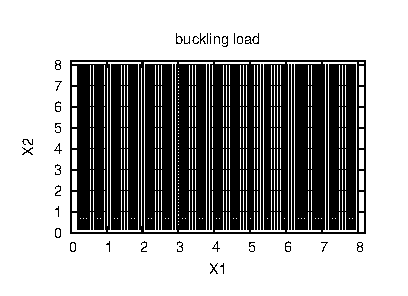
\includegraphics{Const_P.eps}}
%\end{minipage}
%\begin{minipage}[b]{0.5\linewidth}
% \centering
% \resizebox*{7.5cm}{!}{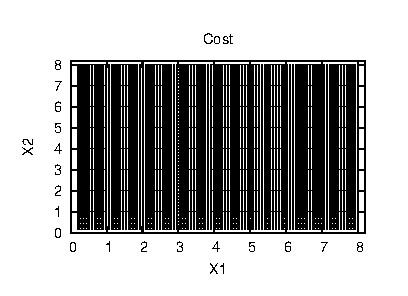
\includegraphics{Const_Price.eps}}
%\end{minipage}
%\begin{minipage}[b]{0.5\linewidth}
% \centering
% \resizebox*{7.5cm}{!}{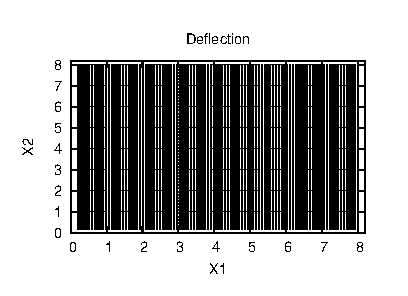
\includegraphics{Const_Dx.eps}}
%\end{minipage}
\begin{minipage}[b]{1\linewidth}
 \centering
 \resizebox*{12cm}{!}{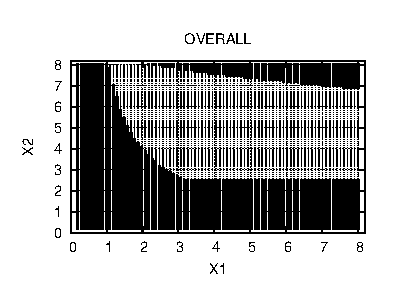
\includegraphics{Const_ALL.eps}}
\end{minipage}

\caption{Investigation of the feasibility of the design $(X_1,X_2)$ plane. The overall feasible design space is presented in the lower right figure with white squares.} 
\label{x1x2}
\end{figure}

%This case was deliberately chosen as a demonstration case due to the clear physical meaning of the relations that appear between its design variables. By carefully examining the objectives it is clear that in order to decrease deflection $X_1$ must be increased(eq. \ref{Deflection}). However any increase in $X_1$ will lead to higher cost (eq. \ref{Cost} ). In order to keep cost stable $X_2$ must simultaneously decrease, this of-course is bounded by the structural constraints (eq. \ref{shear},\ref{bend} and \ref{back}). 
 
Observing the shape of $\Phi$ in figure \ref{reco1}-left it is evident that the problem in hand is, both, extremely anisotropic and non-separable as expected. Using, the proposed in this PhD thesis, variable correlation estimation procedure via applying PCA on the elite-set (fig. \ref{reco1} -right) it is obvious that the principal directions, as they are computed from PCA, are pointing out the separable directions in the design space. The direction with the biggest eigenvalue $e_1$ is the direction that describes the Pareto front, walks along $\Phi=0$. On the other hand the principal direction with the smallest eigenvalue $e_2$ is the direction in the design space that yields the biggest change in $\Phi$ values. Smaller eigenvalue means smaller variance in this direction thus the EA, through its evolution operators, restricted the values of this direction within a small band of values denoting the importance regarding $\Phi$ for the this direction. 

Looking at the physical meaning of the correlations between the design variables in the welded beam case; $e_1$ suggest that if one desires to move along the  $\Phi=0$ front he should either increase $X1$ (welding length) and decrease $X2$ (cross section) or vise vesra. In other words one can move from, say, expensive designs with small deflection to cheap designs with bigger deflection (fig.\ref{Pareto1}) by reducing the cross section but in order to keep respecting the various stress constraints (fig.\ref{x1x2}) one should simultaneously increase the welding length. On the other hand $e_2$ suggest that if one wants to move on the direction that would cause the biggest difference in $\Phi$ he should either increase or decrease both $X1$ \& $X2$ simultaneously.          

\begin{figure}[h!]
\begin{minipage}[b]{1\linewidth}
 \centering
 \resizebox*{!}{4.5 cm}{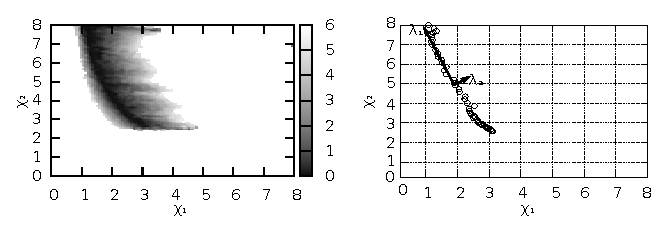
\includegraphics{DOFs.eps}}
\end{minipage}
%\begin{minipage}[b]{0.5\linewidth}
% \centering
%\resizebox*{8cm}{!}{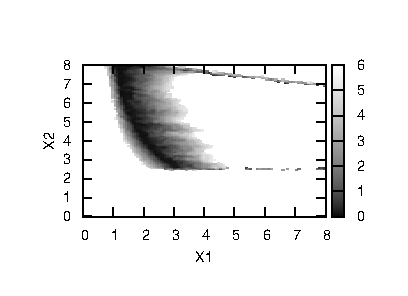
\includegraphics{CaseCorr.eps}}
%\end{minipage}
\caption{Left. $\Phi$ plot over the design space of the welded beam test case. Elite-set plotted on the design space and computed principal directions $e_1$ and $e_2$.} 
\label{reco1}
\end{figure}

\begin{figure}[h!]
\begin{minipage}[b]{1\linewidth}
 \centering
 \resizebox*{!}{6 cm}{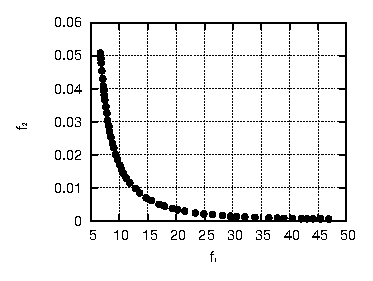
\includegraphics{Pareto.eps}}
\end{minipage}
\caption{Elite-set of fig.\ref{reco1} plotted on the objective space. F1 = cost and F2 = deflection.} 
\label{Pareto1}
\end{figure}


\section{PCA-driven evolution operators} 
%The PCA driven evolution operators to better ``drive'' evolution by utilising the information about the design variable correlations are proposed here as a method to deal with ill-posed optimization problems. To be more specific, PCA is used to identify the relations in the form of direction in the design space. The design space is, then, temporarily aligned with these directions, the necessary evolution operators apply to the so--rotated space and, finally, the generated offspring are transformed back to the original design space. Any sort of dimensionality reduction or rotation of the design space occurs just before (and after) the application of the evolution operators. To initiate PCA, a small number of representative solutions to the problem must be available; this set is dynamically updated during the evolution. In MOO applications, this comprises the members of the current front of non--dominated solutions. In SOO problems, in which there is no set of non--dominated solutions, the principal components can be found by processing a user--defined number of top individuals in the current offspring population. It is evident that, as the evolution proceeds, and the current front of non--dominated solutions converges to the Pareto front, the principal components approach those of the Pareto front. 
In EA-based optimization the application of the evolution operators may benefit a lot from the outcome of the PCA, so as to lead to lower computational cost for the same quality of solutions. To be more specific, PCA is used to identify the directions in the design space that, if used as optimization variables, would lead to an optimization problem with separable objective function. The design space is, then, temporarily aligned with the principal directions and the evolution operators apply to the so--rotated space and, finally, the generated offspring are transformed back to the original design space. The rotation of the design space occurs just before and after the application of the evolution operators and could be combined with truncation, i.e. dimentionality reduction, although this is beyond the scope of this thesis. To perform PCA, a small number of representative solutions to the problem must be available, herein this are the member of the current elite set; this set is dynamically updated during the evolution. In MOO applications, the elite set comprises the members of the current front of non--dominated solutions. In SOO problems, in which there is no set of non--dominated solutions, the principal components can be found by processing a user--defined number of top individuals in the current offspring population. It is evident that, as the evolution proceeds, and the current front of non--dominated solutions converges to the Pareto front, the principal components approach those of the Pareto front. 

Let the aligned with the principal components design vectors \(\vec{x}_i\) be represented by \(\vec{x}^*_i\). The alignment is performed as follows
\begin{equation} 
   \vec{x}^*_i=U(\vec{x}_i-\mu_{X})
   \label{align} %http://users.ics.tkk.fi/jhollmen/dippa/node30.html
\end{equation}
where $\mu_{X}$ is the vector of mean (over the elite set) design variables.
The inverse transformation, from $\vec{x}^*_i$ to $\vec{x}_i$, is given by
\begin{equation} 
   \vec{x}_i=U^{-1}\vec{x}^*_i+\mu_{X}
	\label{re-align}
\end{equation}
It is important to note that the CPU cost to compute \(U^{-1}\) is negligible since U is an orthogonal matrix and, thus, \(U^{-1} = U^T\). 

The two main PCA driven evolution operators, recombination and mutation, are presented below.  

\paragraph{}
\subsection{PCA driven recombination}
In PCA driven recombination, the recombination operator is applied on a continuously updated design space which is sought to be as separable as possible. This, as can be seen in fig.\ref{reco2}, changes the probability of the offspring appearance on the design space in a way that  
yields higher probability to individuals that respect the aforementioned correlations between the design variables (fig.\ref{reco1}). 

\begin{figure}[h!]
\begin{minipage}[b]{0.5\linewidth}
 \centering
 \resizebox*{7cm}{!}{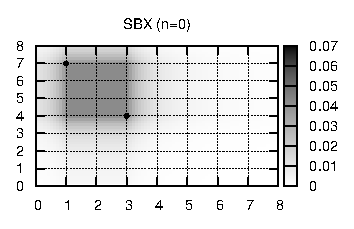
\includegraphics{SBX3dparents2a.eps}}
\end{minipage}
\begin{minipage}[b]{0.5\linewidth}
 \centering
 \resizebox*{7cm}{!}{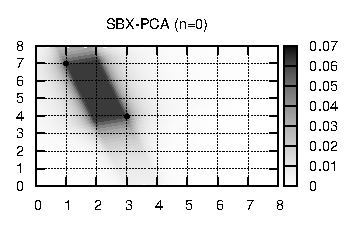
\includegraphics{SBX3dparentsPCAa.eps}}
\end{minipage}
\caption{Offspring appearance probability of the welded beam case, parents are the tow black dots. Left: SBX recombination (section \ref{RecombinationLabel}). Right: PCA driven SBX recombination. The variable correlations (separable directions) for the welded beam case are shown in fig.\ref{reco1}.} 
\label{reco2}
\end{figure}

Observing fig.\ref{reco1} together with fig.\ref{reco2}, it is evident that the proposed method assigns higher probability to the regions near $\Phi=0$ which is the region that accommodates the currently best (elite) individuals. Therefore PCA-driven recombination better achieves its goal of mixing according to the building block hypothesis \cite{Gold89}. Mixing is the process where recombination combines building blocks (low order schemata of high fitness) to form new potentially fit schemata of higher order. The proposed method, simply, increases the probability of the resulting from recombination individuals to be fit.   

%\begin{figure}[h!]
%\begin{minipage}[b]{1\linewidth}
% \centering
% \resizebox*{10cm}{!}{\includegraphics{ellipseturn_eig.eps}}
%\end{minipage}
%\caption{Example $\Phi'$ plot for} 
%\label{phi1}
%\end{figure}


\subsection{PCA driven mutation}
Mutation is also applied on the aligned with principal directions design space. Furthermore the mutation probability on each principal direction is dynamically updated based on the variance ($\vec{V}$) among the members of the elite population on the aforementioned direction ($V(i)$) eq.\ref{alignMut}. This is done in such a way that overall mutation probability per individual is kept constant (and equal to a user defined value) but the way the mutation probability is distributed among the design variable (or, to be more precise, the direction in the design space) is analogous to their importance regarding $\Phi$. As shown through the welded beam case, the importance of each principal direction regarding $\Phi$ is inversely proportional to its eigenvalue/variance therefore the principal direction with higher eigenvalues receive a smaller portion of the overall mutation probability as opposing to the directions with lower eigenvalues that receive a bigger portion of it.        

\begin{equation} 
   P_m^{i}=0.1 P_m + \frac{0.9 P_m N}{P_m^{gl}} (1-\frac{(V(i)-min(\vec{V}))}{(max(\vec{V})-min(\vec{V}))}),~~~~i=1,N 
   \label{alignMut} %http://users.ics.tkk.fi/jhollmen/dippa/node30.html
\end{equation}
where $P_m$ is the user-defined mutation probability, N the number of design variables and 
\begin{equation} 
   P_m^{gl}=\sum^{N}_{i=1} 1-\frac{(V(i)-min(\vec{V}))}{(max(\vec{V})-min(\vec{V}))}
   \label{alignMut2} %http://users.ics.tkk.fi/jhollmen/dippa/node30.html
\end{equation}


The PCA--driven MAEA or MAEA(PCA) (fig.\ref{MAEAPCA2}) algorithm is presented below. 
Let us denote the generation counter by $g$, the number of current entries into the DB by $k_{DB}$ and the minimum number of entries needed to initiate the use of the metamodel--based pre--evaluation phase by $k_{min}$. Then, the steps of the PCA--driven MAEA can be described as follows:
\begin{description}
  \item[Step 1:] For the current offspring population $S^{g}_\lambda$, set $\lambda^*\!=\!\lambda$ (if $k_{DB}\!<\!k_{min}$) or  $\lambda^*\!=\!\lambda_{ex}$ (else). 
  \item[Step 2:] If $k_{DB}\!\ge\!k_{min}$, train $\lambda$ RBF networks on paired input--output patterns selected from the DB, in the vicinity of each offspring. Pre--evaluate the $\lambda$ population members on the so--trained metamodels. Select the $\lambda_{ex}$ top of them, based on dominality and proximity criteria.
  \item[Step 3:] Evaluate the $\lambda_{ex}$ offspring on the problem--specific evaluation software. Update $S^{g}_e$.
  \item[Step 4:] Compute the current set of principal components based on the updated elite set $S^{g}_e$ (eqs. \ref{Cov_Mat} and \ref{spectral}).
  \item[Step 5:] Align the design space to so--computed principal components (eq. \ref{align}). 
  \item[Step 6:] Create the new offspring population $S^{g+1}_\lambda$ through the application of the evolution operator on the aligned individuals. Re--align the generated offspring to the original design space coordinate system,(eq.~\ref{re-align}).
  \item[Step 7:] Set $g\!\leftarrow\!g\!+\!1$; go to step 1.
\end{description}
The above algorithm can readily be transformed to EA(PCA) by eliminating the use of metamodels or by setting $k_{min}$ to a practically infinite number.  
%\figuremacroW{MAEAPCA2}{MAEA-PCA}{Schematic representation of the PCA-driven MAEA algorithm.}{1.0}
%\begin{figure}[h!]
%\begin{minipage}[b]{1\linewidth}
% \centering
% \resizebox*{14cm}{!}{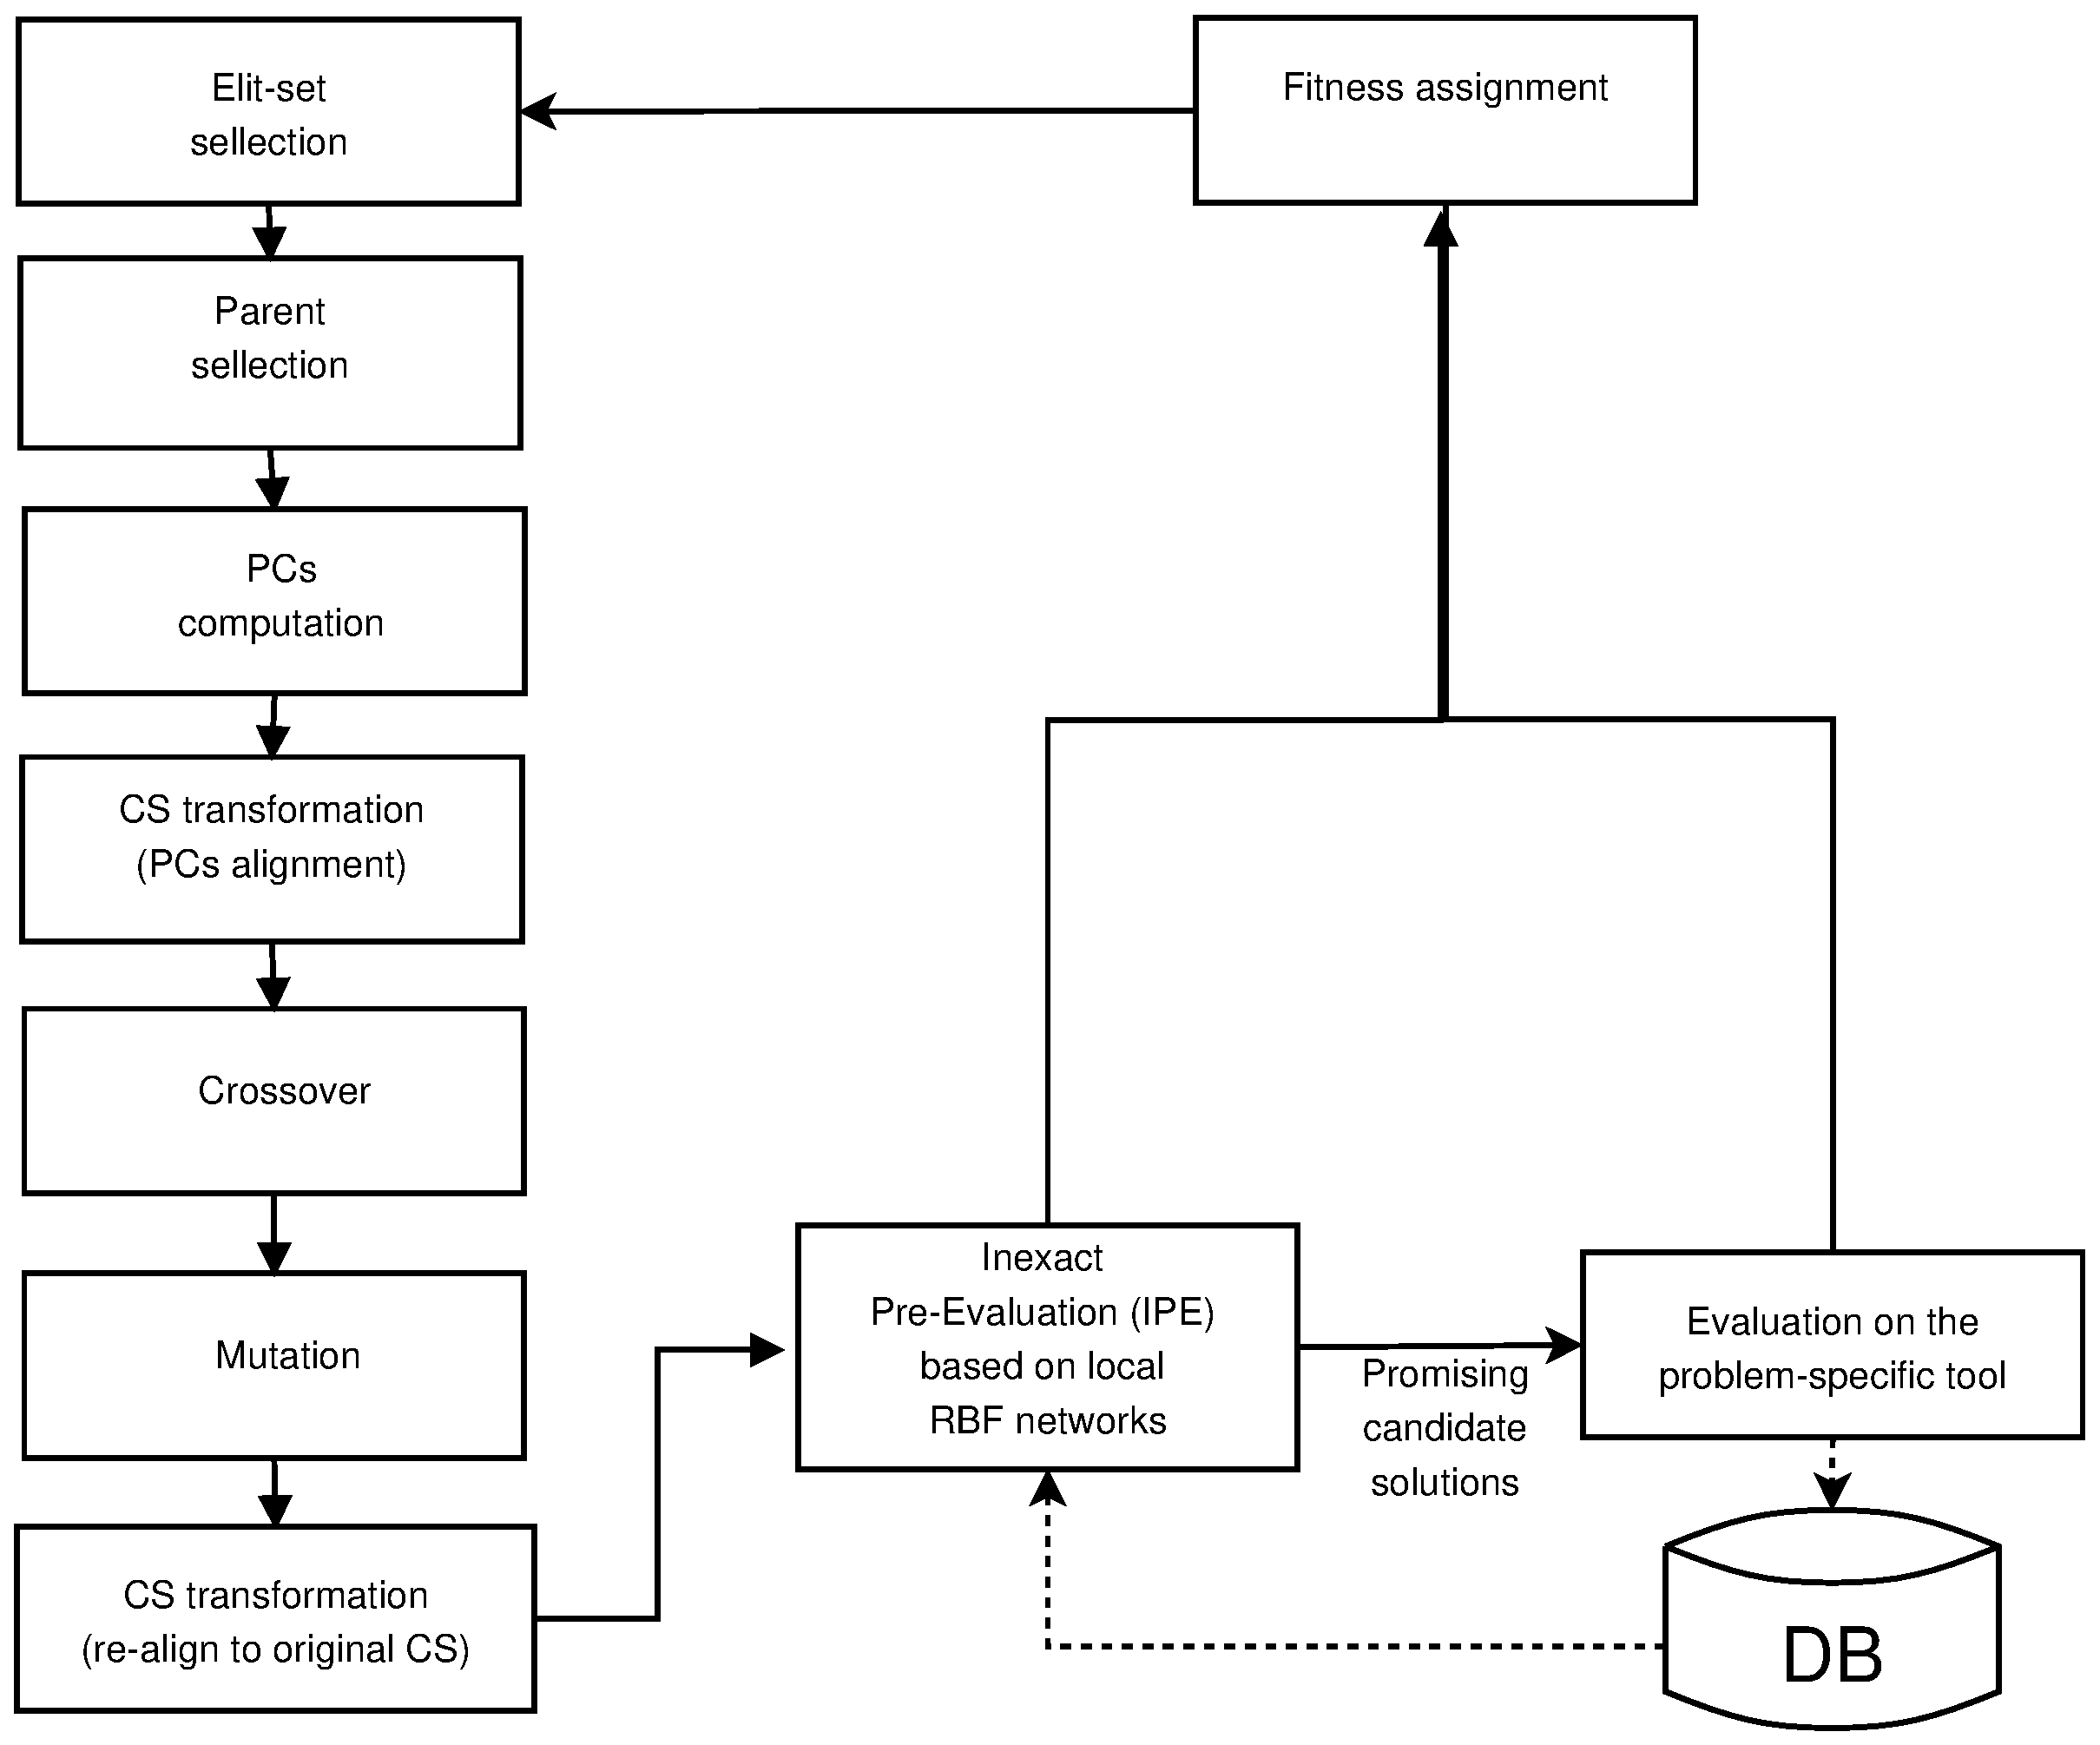
\includegraphics{MAEAPCA2.eps}}
%\end{minipage}
%\caption{Schematic representation of the PCA-driven MAEA algorithm.} 
%\label{MAEAPCA2}
%\end{figure}


%\figuremacroW{HypervolumeComparison}{Hypervolume Comparison}{Hypervolume comparison between EA and EA(PCA), metamodels where not used due to the fast evaluation time of the welded beam case. EA(PCA) outperforms traditional EA even though the dimensionality of the problem in hand is very low.}{0.9}

\subsection{Investigation of the effects of the use of PCA-driven evolution operator in ill-posed optimization problems}

In order to demonstrate the possible performance gain from the use of the PCA-driven EA ten runs for the aforementioned (Welded beam) case and the two mathematical test cases presented in section \ref{Inv2} were performed with different random number generator seeding. The results fo them are presented below. 

Regarding the welded beam test case the average hypervolume indicator in respect to evaluations, over the ten runs, is presented in fig. \ref{HypervolumeComparison}. 

\begin{figure}[h!]
\begin{minipage}[b]{1\linewidth}
 \centering
 \resizebox*{10cm}{!}{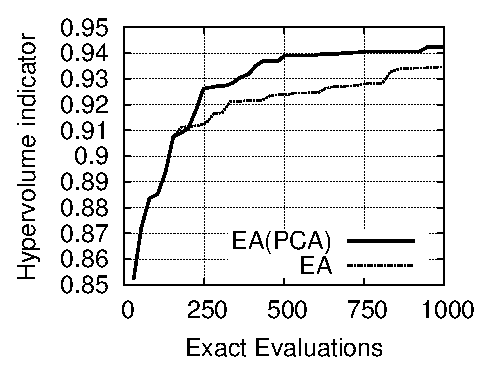
\includegraphics{HypervolumeComparison.eps}}
\end{minipage}
\caption{Hypervolume comparison between EA and EA(PCA), metamodels where not used due to the fast evaluation time of the welded beam case. EA(PCA) outperforms traditional EA even though the dimensionality of the problem in hand is very low.} 
\label{HypervolumeComparison}
\end{figure}

In figure \ref{HypervolumeComparison} one can observe that, even though, the dimension of the problem was deliberately set very low ($N=2$), for observability reasons, something that as shown in section \ref{Inv2} decreases the expected gain from the use of the proposed method. Nevertheless, though, the proposed method still outperforms the traditional EA.  

The comparison between traditional evolution operators and PCA-driven one of the 30D non-separable ellpsoid with $a=1000$ (eq. \ref{ellipse})is presented in fig. \ref{Ellt3}. The plots refer to the mean objective function values of the aforementioned $10$ runs. 

\begin{figure}[h!]
\begin{minipage}[b]{1\linewidth}
 \centering
 \resizebox*{10cm}{!}{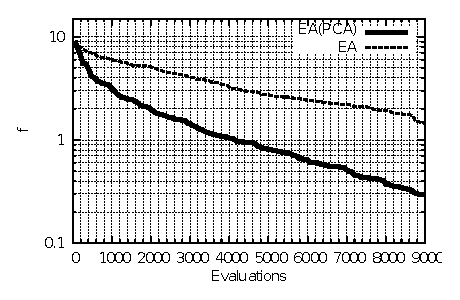
\includegraphics{1000_30d_pca.eps}}
\end{minipage}
\caption{Convergence comparison between for the 30D ellipsoid case (eq. \ref{ellipse}) with condition number ($a = 1000$). The proposed PCA-driven evolution operators significantly outperform the traditional ones.} 
\label{Ellt3}
\end{figure}

In figure \ref{Ellt3} one can observe the significant gain from the use of the proposed method in comparison with a traditional EA in the 30D ellipsoid case.

Regarding the multi-dimensional and multi-modal test case of eq.\ref{mm}, comparison between PCA-driven and traditional evolution operators are presented in the 30D version in fig.\ref{mmt3}.  

\begin{figure}[h!]
\begin{minipage}[b]{1\linewidth}
 \centering
 \resizebox*{10cm}{!}{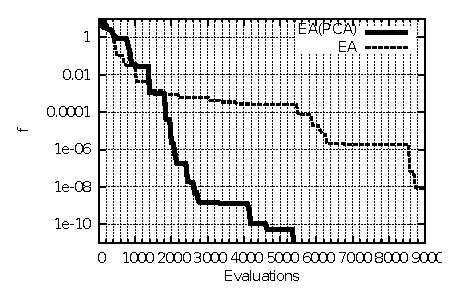
\includegraphics{30d_pca.eps}}
\end{minipage}
\caption{Convergence comparison between for the 30D multi-modal case (eq. \ref{mm}). The proposed PCA-driven evolution operators significantly outperform the traditional ones.} 
\label{mmt3}
\end{figure}

In figure \ref{mmt3} one can observe that the use of PCA-driven evolution operators significantly enhances the EA efficiency.

\FloatBarrier
\section{EAs assisted by PCA-assisted metamodels}
The main challenge regarding the use of artificial neural networks as metamodels in MAEAs is to overcome the so--called ``curse of dimensionality'', when handling problems with a large number of design variables. 
The number of training patterns required in order to build a reliable metamodel increases in parallel with the problem dimensionality; a side--effect is that its training becomes computationally costly. On the other hand the need for more training patterns per metamodel delays the application of the IPE phase during the MAEA, until the DB has a substantial number of entries, something that leads to a further increase of the wall clock time of the optimization.

This thesis proposes the appropriate reduction the number of the RBF network sensory (input) nodes and, consequently, the required number of training patterns. The eigenvectors computed through the PCA are associated with the variance of the objective function. 
If the elite set is expressed in a coordinate system aligned with the principal components, any plot of the objective function in terms of the first components (i.e. those with higher variance), must be scattered enough. In contrast, along the directions with small variances, the elite members are almost not scattered at all. 

The proposed method takes advantage of the above and cuts off a preselected number of the RBF network sensory units, particularly those related to the higher variances directions of the design space. As a result, the RBF network will be trained on lower dimension data. 
This truncation is applied only during the RBF network training, by firstly rotating/aligning all the selected training patterns with the eigenvectors and, then, cutting off those sensory nodes corresponding to the higher eigenvalues. 
    
% The use of the IPE technique, in its standard form, would require the use of RBF networks with two sensory nodes each, trained on neighbouring to the candidate solution, already evaluated stored individuals as shown in figure \ref{2dann}. 
    
    
%\begin{figure}[h!]
%\begin{minipage}[b]{1\linewidth}
% \centering
% \resizebox*{15cm}{!}{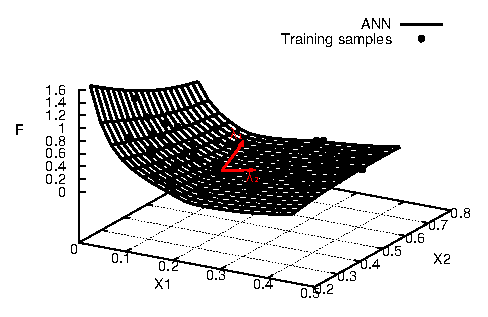
\includegraphics{2dANN.eps}}
%\end{minipage}
%\caption{Welded beam test problem: ANN with two sensory node used as metamodel in the standard IPE form. The ANN prediction is plotted as a surface grid and the training patterns used for its training as dots.} 
%\label{2dann}
%\end{figure}

\begin{figure}
\begin{minipage}{0.48\textwidth}
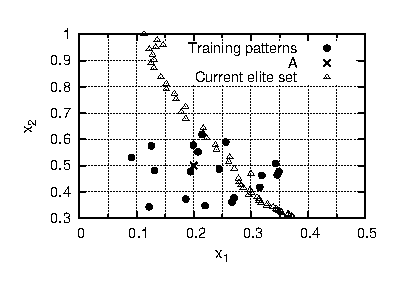
\includegraphics[scale=1.2]{IPE/x1_x2.eps}
\end{minipage}
\begin{minipage}{0.48\textwidth}
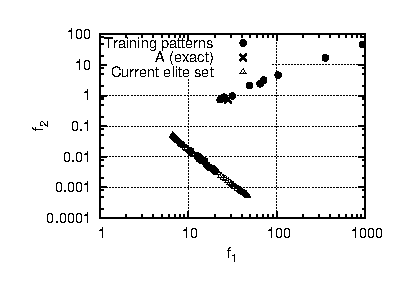
\includegraphics[scale=1.2]{IPE/f1_f2.eps}
\end{minipage}
\caption{Welded beam test problem: An instance of the evolution process, where the current elite set, a candidate solution (A) and the training patterns selected from the current DB for the metamodel to be built at A are plotted in the design (left) and objective (right) space.}
\label{fig:f1f2}
\end{figure}

Figure \ref{fig:f1f2} presentation of an instance of the evolution process, namely at the end of the $6^{\mbox{th}}$ generation. At this instance, $\lambda$ new offspring have just been generated. Let us assume that the candidate solution A, with $(x_1, x_2)\!=\!(0.2,0.5)$  shown in Figure \ref{fig:f1f2}, needs to be approximately (``inexactly'' ) pre--evaluated using an appropriately trained local RBF network. 
For this purpose, $19$ patterns are selected from the DB. 
In Figure \ref{fig:f1f2}, the training patterns, the candidate solution and also the current elite set are plotted both in the design ($x_1, x_2$) and objective ($f_1, f_2$) spaces. 
The exact values of $f_1$ and $f_2$ for A are also shown.
It is evident that, in a problem with only two design variables, there is no reason to reduce the number of design variables during the training of the RBF networks. However, we do so, just for the purpose of demonstration.  

\begin{figure}
\begin{minipage}{0.48\textwidth}
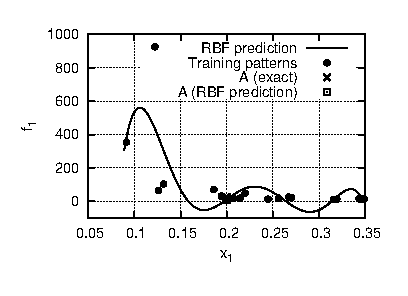
\includegraphics[scale=1.2]{IPE/f1_x1.eps}
\end{minipage}
\begin{minipage}{0.48\textwidth}
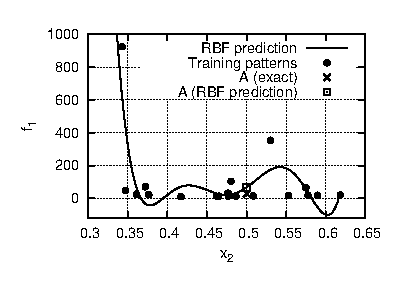
\includegraphics[scale=1.2]{IPE/f1_x2.eps}
\end{minipage}
\caption{Welded beam test problem: RBF predictions of $f_1$ if $x_1$ (left) and $x_2$ (right) are separately applied to the single sensory unit of the network. }
\label{fig:f1x1x2}
\end{figure}

\begin{figure}
\begin{minipage}{0.48\textwidth}
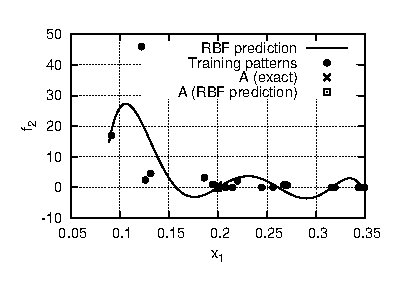
\includegraphics[scale=1.2]{IPE/f2_x1.eps}
\end{minipage}
\begin{minipage}{0.48\textwidth}
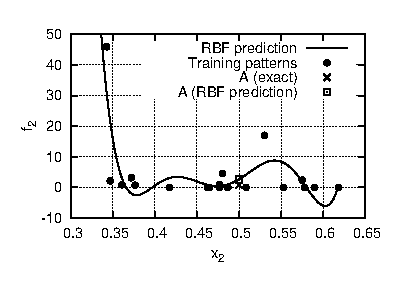
\includegraphics[scale=1.2]{IPE/f2_x2.eps}
\end{minipage}
\caption{Welded beam test problem: RBF predictions of $f_2$ if $x_1$ (left) and $x_2$ (right) are separately applied to the single sensory unit of the network. }
\label{fig:f2x1x2}
\end{figure}

A first demonstration of the proposed method will be based on the welded
beam problem (figure \ref{case}). In Figure \ref{fig:f1x1x2}, the $f_1$ predictions using two RBF networks, with either $x_1$ or $x_2$ as the only sensory unit of each network, are shown. Though these networks, after being trained on the selected $19$ patterns must be used to predict the objective functions only at A, it presents certain interest to observe the overall deviation between the continuous line which stands for the network response and the training patterns' responses. 
Recall that the number of RBF centers is less than the number of training parameters, so the network does not interpolate the training patterns.
The observed high deviations, which could be even higher for some other candidate solutions, are easily explained by the fact that a two-variable function $f_1(x_1,x_2)$ is handled as $f_1(x_1)$ or $f_1(x_2)$. The corresponding results for $f_2$, instead of $f_1$, are shown in Figure \ref{fig:f2x1x2}. 
The exact objective function values at A along with the RBF predictions are tabulated in table \ref{tab:f1f2x1x2}. As it can be seen from this table, $f_1$ is predicted with a relative error of about $57\%$ if $f_1\!=\!f_1(x_1)$ and $138\%$ if $f_1\!=\!f_1(x_2)$ and the error of $f_2$ is about $110\%$ if $ f_2\!=\!f_2(x_1)$ and $260\%$ if $ f_2\!=\!f_2(x_2)$.


\begin{figure}
\begin{minipage}{0.48\textwidth}
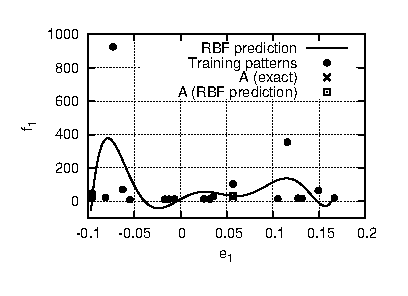
\includegraphics[scale=1.2]{IPE/f1_e1.eps}
\end{minipage}
\begin{minipage}{0.48\textwidth}
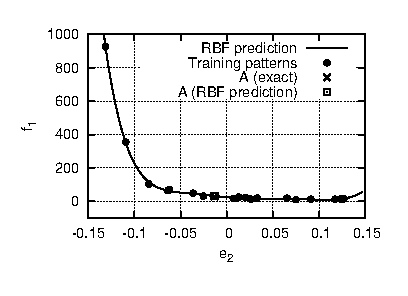
\includegraphics[scale=1.2]{IPE/f1_e2.eps}
\end{minipage}
\caption{Welded beam test problem: RBF predictions of $f_1$ if $e_1$ (left) and $e_2$ (right) are separately applied to the single sensory unit of the network.}
\label{fig:f1e1e2}
\end{figure}

\begin{figure}
\begin{minipage}{0.48\textwidth}
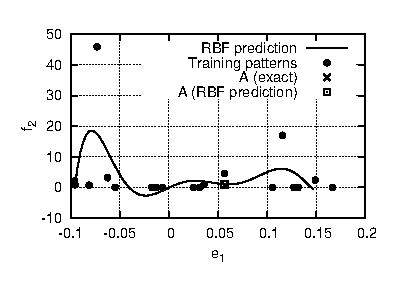
\includegraphics[scale=1.2]{IPE/f2_e1.eps}
\end{minipage}
\begin{minipage}{0.48\textwidth}
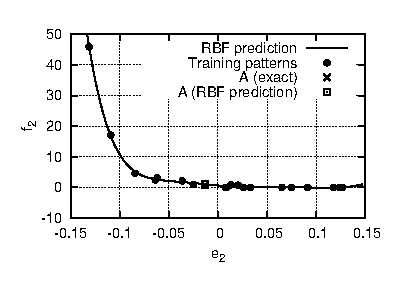
\includegraphics[scale=1.2]{IPE/f2_e2.eps}
\end{minipage}
\caption{Welded beam test problem: RBF predictions of $f_2$ if $e_1$ (left) and $e_2$ (right) are separately applied to the single sensory unit of the network. }
\label{fig:f2e1e2}
\end{figure}

\begin{table}[h!]
\begin{center}
\begin{tabular}{c  c | c | c}
		&      Exact  	 		&  RBF--based predictions    &  RBF--based  predictions   \\
		&  $(f_1,f_2)$ values   &  assuming $f_i=f_i(x_1)$    &   assuming $f_i=f_i(x_2)$  \\
		\hline
$f_1$	& $28.07$   &      $11.88$     &      $66.9$        \\
$f_2$	& $0.73$     &      $-0.08$     &      $2.66$        \\
\end{tabular}
\end{center}
\caption{Welded beam test problem: Exact response and RBF predictions of $f_1$ and $f_2$ at A, using either $x_1$ or $x_2$ as the only input to the network.}
\label{tab:f1f2x1x2}
\end{table}


The PCA of the current elite set is used to compute the two principal components which, in turn, are used to select the single variable that must preferably be associated with the only sensory unit of the RBF network. The design space is transformed according to the computed principal components and the RBF training is repeated using either $e_1$ or $e_2$, instead of $x_1$ and $x_2$, as input. 
The RBF networks' predictions are shown in Figures \ref{fig:f1e1e2} and \ref{fig:f2e1e2} and Table \ref{tab:f1f2e1e2}. 
In particular, $f_1$ is predicted with a relative error of about $17\%$ if $f_1\!=\!f_1(e_1)$ and $13\%$ if $f_1\!=\!f_1(e_2)$ and $f_2$ with about $41\%$ if $f_2\!=\!f_2(e_1)$ and $43\%$ if $f_2\!=\!f_2(e_2)$. From these figures, it can be concluded that the RBF networks can be trained only on $e_2$, i.e. the principal component with the smaller variance, since the training patterns are less scattered both in ($f_1,e_2$) and ($f_2,e_2$) and the obtained prediction trend is more confident.




\begin{table}[h!]
\begin{center}
\begin{tabular}{c  c | c | c}
		&      Exact  	 		&  RBF--based predictions    &  RBF--based  predictions   \\
		&  $(f_1,f_2)$ values   &  assuming $f_i=f_i(e_1)$    &   assuming $f_i=f_i(e_2)$  \\
		\hline
$f_1$	& $28.07$   &      $32.86$     &      $31.84$        \\
$f_2$	& $0.73$     &      $ 1.04$     &       $ 1.06$        \\
\end{tabular}
\end{center}
\caption{Welded beam test problem: Exact responses and RBF predictions of $f_1$ and $f_2$ at A, using either $e_1$ or $e_2$ as the only input to the network.}
\label{tab:f1f2e1e2}
\end{table}


%stelios 
\subsection{Investigation of the effects of the use of PCA assisted metamodels in ill-posed optimization problems}

To demonstrate the possible performance gain from the use of the proposed PCA assisted metamodels 10 runs for the two mathematical test cases presented in section \ref{Inv2} were performed with different random number generator seeding. The results of them are presented below. 

Regarding comparison between traditional metamodels using PCA only to drive the evolution operators (MAEA(PCA)) and PCA assisted metamodels  or M(PCA)AEA(PCA) of the 30D non-separable ellpsoid with $a=1000$ (eq. \ref{ellipse}) is presented in fig. \ref{Ellt3-m}. The plots refer to the mean objective function values of the aforementioned $10$ runs. IPE phase for MAEA(PCA) initiated after $300$ individuals where stored in the database and $25$ to $29$ training patterns, in the $\Re^{30}$ space, where used to train the RBF networked employed as metamodel. Regarding the M(PCA)AEA(PCA), IPE phase started after only $100$ individuals where stored in the database since only $4$ to $8$ training patterns, in the truncated  $\Re^{10}$  space, where required for the RBF network training. The $\Re^{10}$ is comprised by the $10$ most important directions in the design space according to method proposed above. 

\begin{figure}[h!]
\begin{minipage}[b]{1\linewidth}
 \centering
 \resizebox*{10cm}{!}{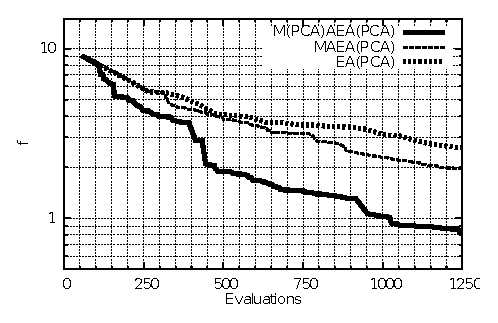
\includegraphics{1000_30d_pca_ipe.eps}}
\end{minipage}
\caption{Convergence comparison between for the 30D ellipsoid case (eq. \ref{ellipse}) with condition number ($a = 1000$). The proposed M(PCA)AEA(PCA) method outperform the MAEA(PCA) one.} 
\label{Ellt3-m}
\end{figure}


Regarding the multi-dimensional and multi-modal test case of eq.\ref{mm}, comparison between MAEA(PCA) and M(PCA)AEA(PCA) are presented for the 30D version in fig.\ref{mmt3m}. Regarding MAEA(PCA)  IPE phase initiated after $300$ individuals where stored in the date base and $15$ to $19$ training patterns, in the $\Re^{30}$ space, where used to train the  metamodel. As far at the M(PCA)AEA(PCA) is concerned, the training pattern dimension was truncated from $30$ to the $10$ most important regarding $f$. That allowed for the  IPE phase to start after only $100$ individuals where stored in the database since only $5$ to $9$ training patterns where required for the RBF network training.

\begin{figure}[h!]
\begin{minipage}[b]{1\linewidth}
 \centering
 \resizebox*{11cm}{!}{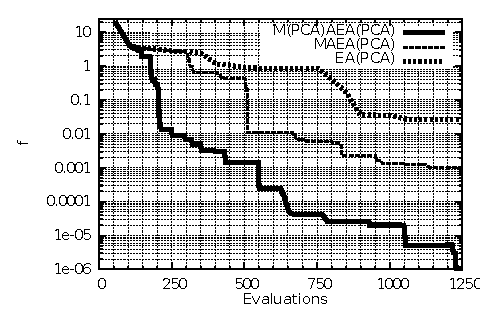
\includegraphics{30d_pca_ipe.eps}}
\end{minipage}
\caption{Convergence comparison between for the 30D multi-modal case (eq. \ref{mm}).The proposed M(PCA)AEA(PCA) method outperform the MAEA(PCA) one.} 
\label{mmt3m}
\end{figure}

In figures \ref{Ellt3-m} and \ref{mmt3m} one can observe that the use of PCA assisted metamodels further enhances the MAEA efficiency.

%stelios

\section{Design of a compressor cascade using the proposed M(PCA)AEA(PCA) method}


The design of a two dimensional compressor cascade operating at $M_1=0.54$, $a_1=44^o$ and $Re=4\times10^5$ for minimum total pressure losses ($\omega$) eq.\ref{omegaLosses} is sought. 

The blade airfoil is designed subject to a number of aerodynamic and geometrical constraints: the optimal airfoil must turn the flow by more than $30^o$ and ensure that its thickness at three chord-wise positions ($0.3c$, $0.6c$ \& $0.9c$) must be greater that ($0.10c$, $0.08c$ \& $0.01c$)  respectively.     

The airfoil shape is parameterized based on a mean-camber line and thickness distributions scheme as presented in section \ref{Drela1}, a parameterization that yields $27$ design variables.

The merits of the proposed M(PCA)AEA(PCA) method will be examined through the comparison of a traditional MAEA against a M(PCA)AEA(PCA) where PCA is used both to drive the evolution operators and also during the IPE phase to reduce the metamodel dimension. The populations for both MAEAs are $\mu=20$, $\lambda=60$ and $\lambda_e=6$. Both cases use local RBF networks as metamodels trained on a small number of automatically selected training patterns. The MAEA uses a number of  $20$ to $30$ training patterns in the $\Re^{27}$ space. IPE phase for MAEA starts after $400$ individuals are stores in the database. Regarding M(PCA)AEA(PCA) the RBF networks used as metamodels are trained with $5$ to $8$ training patterns in the reduced as presented above $\Re^{10}$ space. The reduced dimension makes possible the use of metamodels significantly earlier, the IPE phase for M(PCA)AEA(PCA) starts after only $200$ individuals are stored in the database. 


\begin{figure}[h!]
\begin{minipage}[b]{1\linewidth}
 \centering
 \resizebox*{11cm}{!}{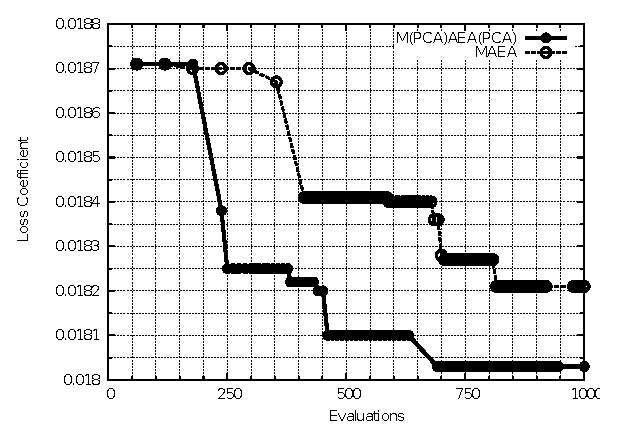
\includegraphics{CompPCA.eps}}
\end{minipage}
\caption{Convergence comparison between MAEA and M(PCA)AEA(PCA) methods.} 
\label{PCADrelaRes}
\end{figure}

Figure \ref{PCADrelaRes} shows the convergence of both methods. M(PCA)AEA(PCA) outperforms the traditional MAEA during all but the initial steps of the optimization procedure. 

\begin{figure}[h!]
\begin{minipage}[b]{1\linewidth}
 \centering
 \resizebox*{16cm}{!}{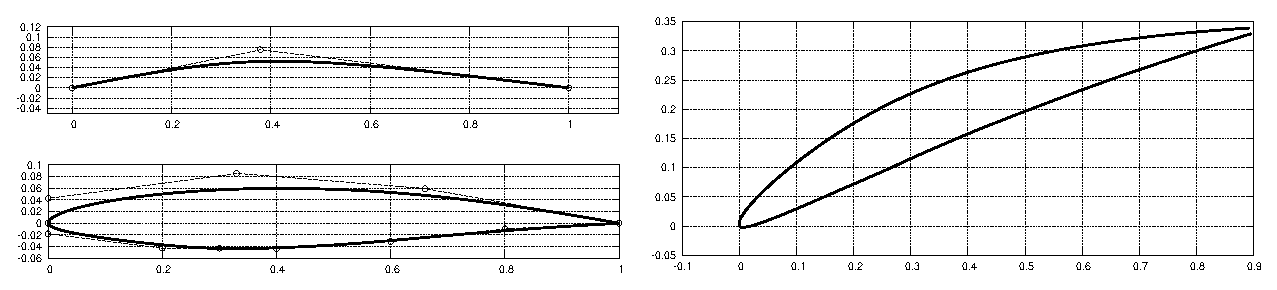
\includegraphics{ResD.eps}}
\end{minipage}
\caption{The optimal airfoil resulting form M(PCA)AEA(PCA). Left: mean camper line and thickness distribution together with their control polygons. Right: The final airfoil after superimposing thickness distribution on the mean camper line and turned accordingly with the stagger angle.} 
\label{PCADrelaRes}
\end{figure}

The optimal airfoil resulting form M(PCA)AEA(PCA) (fig. \ref{PCADrelaRes}) has total pressure losses $\omega=0.01803$ and respects both the thickness and flow turning constraints.  Flow turning of the blade in hand is $\Delta a=30^o$

\begin{figure}[h!]
\begin{minipage}[b]{1\linewidth}
 \centering
 \resizebox*{12cm}{!}{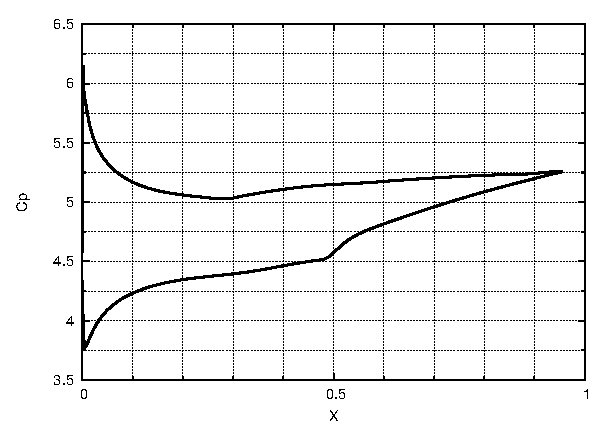
\includegraphics{Best_CP_PCA.eps}}
\end{minipage}
\caption{Pressure coefficient $C_p$ of the optimal airfoil fig.\ref{CBRDrelaRes}.} 
\label{PCADrelaRes_cp}
\end{figure}

% ---------------------------------------------------------------------------
% ----------------------- end of thesis sub-document ------------------------
% ---------------------------------------------------------------------------